\documentclass[10pt, letterpaper, headings=Large, DIV=14]{scrartcl}
\usepackage{graphicx}
\usepackage{amssymb}
\usepackage{epstopdf}
\DeclareGraphicsRule{.tif}{png}{.png}{`convert #1 `dirname #1`/`basename #1 .tif`.png}

% \usepackage{titlesec}
% \titleformat{\subsection}[runin]{\sffamily \bfseries \large}{}{}{}[]
\renewcommand*{\titlepagestyle}{scrheadings}
\usepackage{aas_macros}
\usepackage{palatino}
\usepackage{multicol}
\usepackage[]{natbib}
\bibstyle{apj}
\usepackage{amssymb}

\usepackage[usenames,dvipsnames,svgnames,html]{xcolor}
\usepackage{setspace}  % Needed for Double Spacing
\usepackage[english]{babel}
\usepackage{lipsum}

\DeclareGraphicsRule{.tif}{png}{.png}{`convert #1 `dirname #1`/`basename #1 .tif`.png}
\usepackage{hyperref}

%\title{Galaxy evolution through the lens}  % add title here
%\author{T. Emil Rivera-Thorsen}  % include Author's name here
\date{}                                           % Activate to display a given date or no date

%%% BEGIN HYPERREF
\hypersetup{
	colorlinks=true,
	linkcolor=blue,
	urlcolor=blue,
	citecolor=black,
}
%%% END HYPERREF


%%% BEGIN KOMASCRIPT
\setkomafont{title}{\large \sffamily \bfseries \color[HTML]{1F78B4}}
\setkomafont{captionlabel}{\small \bfseries \sffamily}
\setkomafont{caption}{\footnotesize}
\setcapindent{1em}
\setkomafont{section}{\large \color[HTML]{1F78B4}}
\setkomafont{subsection}{\normalsize \color[HTML]{000000}}
\setkomafont{author}{\small \itshape}
\setkomafont{pagenumber}{\large \upshape \bfseries \color[HTML]{FFFFFF}}
\usepackage[automark]{scrpage2}
\pagestyle{scrheadings}
\setheadsepline{.0pt}
\clearscrheadings
\automark[section]{chapter}
\ihead{\upshape \color[HTML]{999999} T. Emil Rivera-Thorsen}
\ohead{\colorbox[HTML]{1F78B4}{\color{white} \pagemark}}
\chead{\upshape \color[HTML]{999999} Research and interests}
\cfoot{}

%%% END KOMASCRIPT
\begin{document}

% \maketitle
\noindent {\color[HTML]{1F78B4}\sffamily \bfseries \Large 
Research and interests}

\section*{Overview}

Throughout my Ph.D., my work has been focused on optical and UV spectroscopy of
the ISM and CGM of local-Universe starburst galaxies. This I have studied in
ionized and neutral metal absorption lines in the UV with HST-COS to investigate
the impact of ISM kinematics and geometry on Ly$\alpha$ radiative transfer and
escape \citep[see ][]{RiveraThorsen2015} and Lyman Continuum escape
(Rivera-Thorsen et al. \emph{a}, submitted). I have analyzed NUV/optical nebular
emission lines from the galaxies in the sample of \cite{RiveraThorsen2015} in
archival spectra from SDSS \citep{LARSI}, and in high detail in spatially
resolved VLT/X-Shooter slit spectra (Rivera-Thorsen et al. \emph{b}, submitted).

The latter project has led to my interest being turned in the direction of
(low-luminosity or obscured) AGN due to what we believe is the serendipitous
discovery of an LLAGN in the galaxy Haro 11, which is otherwise by optical line
ratios classified as a pure starburst galaxy. A shift in direction towards AGN
outflows therefore seems to make a lot of sense, as I have a large skill set and
experience in ISM/CGM kinematics and other diagnostics which require no or
little tweaking, and I have a rapidly growing interest in the field.

Below, I shall present these main topics in more depth. In addition, I have been
involved in smaller projects; I have received training and taken part in the
reduction and cleaning of 21 cm.\ radio interferometric data from the Karl I.
Jansky Very Large Array (VLA) of LARS galaxies treated in \cite{LARSIII}; I have
reduced VLT/X-Shooter data for \cite{Sandberg2013} and \cite{Stritzinger2014},
and performed NUV/Optical observations with the Nordic Optical Telescope on La
Palma, Spain, for \cite{Sandberg2015} and other projects.



\section*{The Lyman Alpha Reference Sample + local Lyman continuum leakers}

The Lyman Alpha Reference Sample \citep[LARS,][]{LARSI,LARSII} is a sample of 14
+ 28 star-forming galaxies at low redshifts, selected for high star formation. I
led an analysis of HST-COS spectra of the sample galaxies focusing on the
kinematics and geometrical configuration of the neutral ISM\@. We computed
systemic velocities of the sample galaxies from re-measured nebular emission
lines in SDSS spectra of the sample galaxies \citep[a number of galaxy
properties like metallicity etc.\ derived from these lines were published in the
first LARS paper ]{LARSI}, and measured bulk in-/outflows of the neutral and hot
ISM from, mainly, Si \textsc{ii} and Si \textsc{iv} absorption lines.

We applied the Apparent Optical Depth method
\citep[e.g.]{Savage1991,Pettini2002,Quider2009} as implemented by
\cite{Jones2013}, to disentangle opacity and covering fraction of the neutral
gas in metal absorption lines. This method allows a mapping of covering
fractions in velocity space,$f_C (v + \delta v)$, by utilizing multiple lines
rising from the same ground state of an ion, in this case Si \textsc{ii}. In the
optically thin limit, the relative depths of these lines are a simple reflection
of the lines' oscillator strengths $f\lambda$; but as the column density of the
ion grows, the lines grow optically thick, in which case they all have the same
depth which reflects the covering fraction of the gas in which they reside. In
all cases, both the extremes mentioned above and in intermediate cases, the
residual intensity $I/I_0$ in any given as a function of $f\lambda$, column
density $N$ and overing fraction\footnote{of gas \emph{with velocities within
the bin}.} can be fitted to the observed values of $I/I_0$ and tabular values of
$f\lambda$, and best-fit values of $N$ and $f_C$ found for the given bin. 


\begin{figure}[h] %  figure placement: here, top, bottom, or page
   \centering
   \includegraphics[width=\textwidth]{./AOD-details-example-4pane.pdf} 
   \caption{Illustration of the AOD method with example data from Haro 11.
   \textbf{Far left}: Line profile of Si\textsc{ii}\(\lambda\lambda 1260, 1304,
   1526\), and a vertical red line denoting the velocity bin of interest for the
   example. \textbf{Center left}: Residual intensity as a function of
   \(f\lambda\) for the three lines. The best fit of \(I/I_0(f\lambda)\) is 
   shown in magenta. In gray is shown for illustration \(I/I_0\) in the extreme
   cases of \emph{a)} unchanged $f_C$ but much higher $N$ (dotted) or \emph{b)}
   $f_C=1$ and $N$ 0.5 dex lower. \textbf{Center right}: $\log N$ as function of
   $v$ for these profiles, and \textbf{far right}: $1-f_C$ as function of v
   (orange circles) superimposed on the profile of Si \textsc{ii} 1260 (black
	   steps). Shaded regions are standard errors. }
   \label{fig:AOD}
\end{figure}

The method is illustrated in Fig.~\ref{fig:AOD} with data for Haro 11 from
Rivera-Thorsen et al. \emph{a}, where the leftmost panel shows the measured
values for three lines, and the red line indicates the bin of interest. Center
left panel shows, as black dots, the residual intensities of the lines of the
leftmost panels plotted against $f\lambda$, with the best-fit function shown as
a magenta curve. In gray is shown the same function with $N$ and $f_C$ varied
for illustrative purposes. The center-right panel shows the computed values of
$\log N$, and the far-right shows $1-f_C$ plotted in orange on top of the line
profile of Si \textsc{ii}, which unlike the other two lines is found to be
optically thick everywhere. One should note that since gas at different
velocities generally does not occupy the same projected area, $f_C$  only
provides a lower limit to the total covering fraction. However, a low $f_C$ max
may imply a higher probability of finding direct sight lines through the neutral
medium.  See RT15 for details. 

We finally compared the properties found through spectroscopy, to global
properties derived from HST-ACS imaging \citep{LARSII} and VLA 21 cm HI radio
interferometry \citep{LARSIII}. Interestingly, we found a strong anticorrelation
between $f_{C, \mathrm{max}}$ and H$\alpha$ equivalent width. We tentatively
interpreted this as indicating that feedback from strong star formation activity
may drive Rayleigh-Taylor instabilities in the outflowing medium, causing it to
fragment. 
% An analysis of this kind , but of a larger sample of local galaxies,
% is a main pillar in both the proposed Hubble Legacy sample and the
% SAFE sub-projects in this
% proposal. 
Combined with insights about the connection between Ly$\alpha$
emission and Lyman Continuum continuum \citep[e.g.][]{Verhamme2015}, this method
has also allowed us to constrain the ISM models consistent with Lyman Continuum
escape in Tololo 1247-232 (Puschnig et al., submitted) and Haro 11
(Rivera-Thorsen et al \emph{a}). 


\section*{Spatially and kinematically resolved spectroscopy}

Another main project of mine has consisted in a spatially-resolved, high-detail
analysis of UV/Optical VLT/X-Shooter slit spectra of the recombination nebulae
surrounding three starburst regions in nearby galaxies ESO 338-IG04 and Haro 11.
The spectra, obtained as part of the X-Shooter Science Verification Program in
2009, were of a high enough S/N ratio that each pixel row could be extracted and
measured as an individual spectrum. For each of these, the H$\alpha$ line was
then modeled with 1-5 Gaussian emission line components, constrained such that
components must be coherent between neighboring spatial regions. Components
which behaved coherently over spatial regions larger than the seeing were then
interpreted as originating in the same physical subsystem, assigned an
identifying label and grouped this way. 

\begin{figure}[h] %  figure placement: here, top, bottom, or page
   \centering
   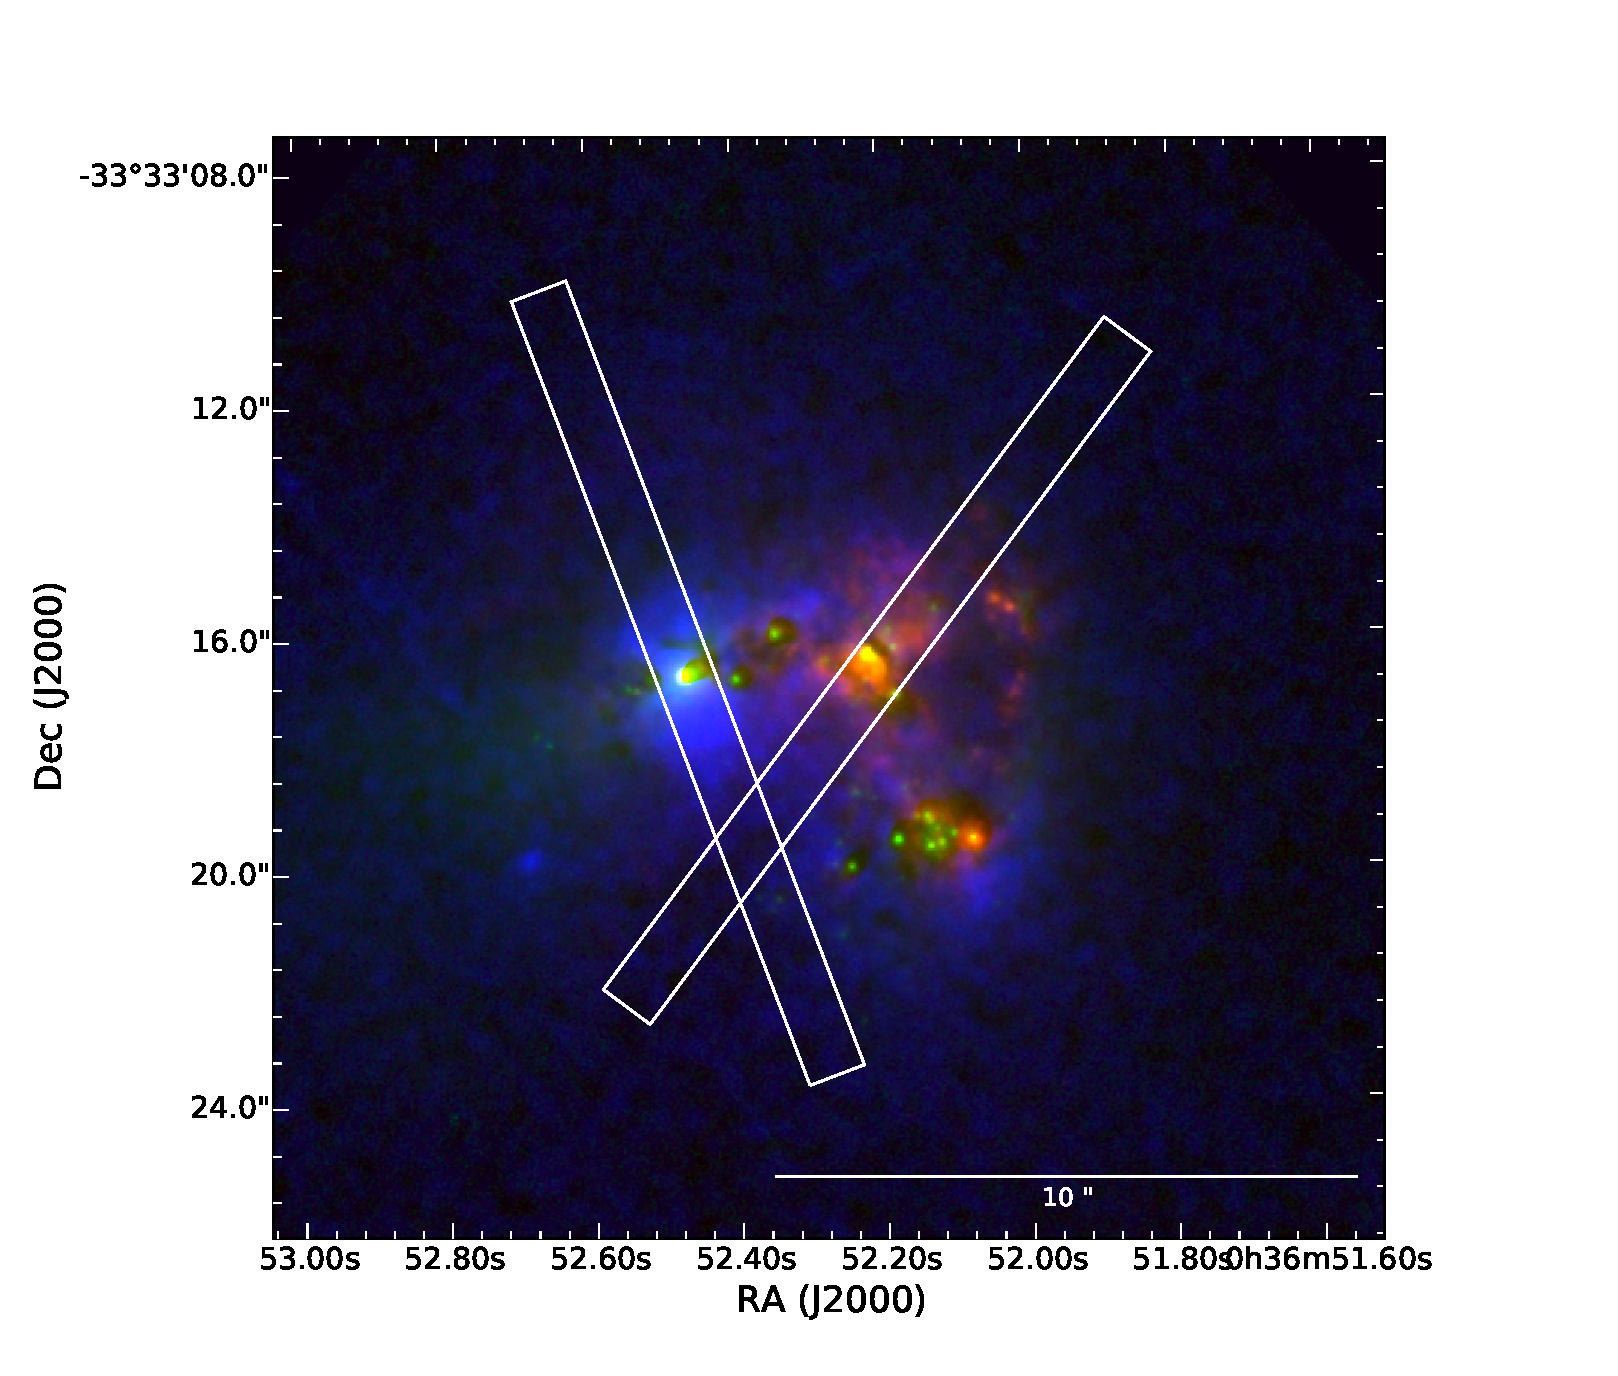
\includegraphics[width=0.27\textwidth]{Haro11-slit.pdf}
   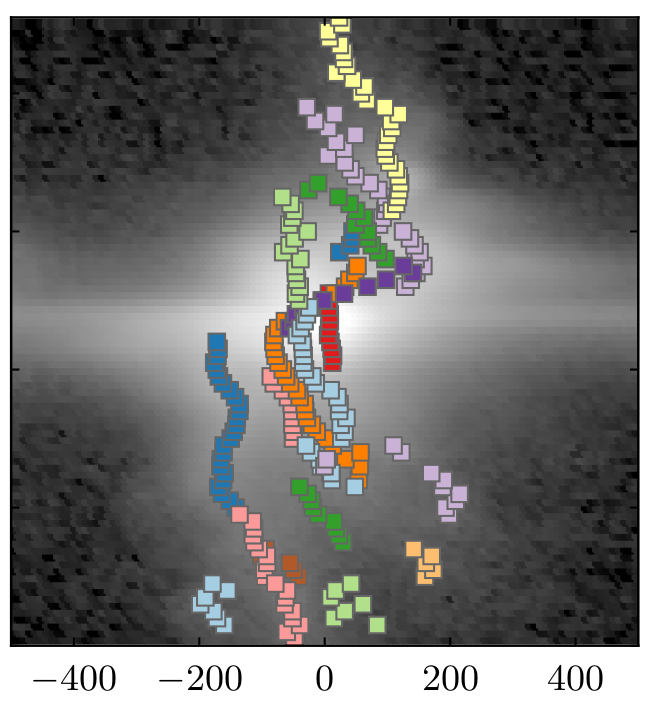
\includegraphics[width=0.19\textwidth]{Selection_204.png} 
   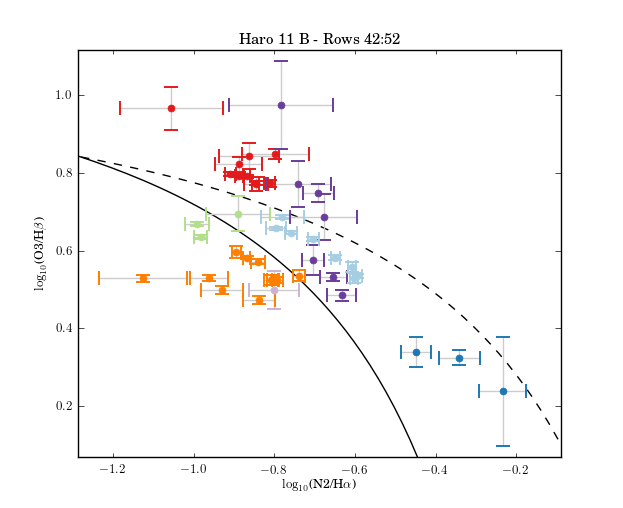
\includegraphics[width=0.27\textwidth]{BPT-HaroB-Center.png} 
   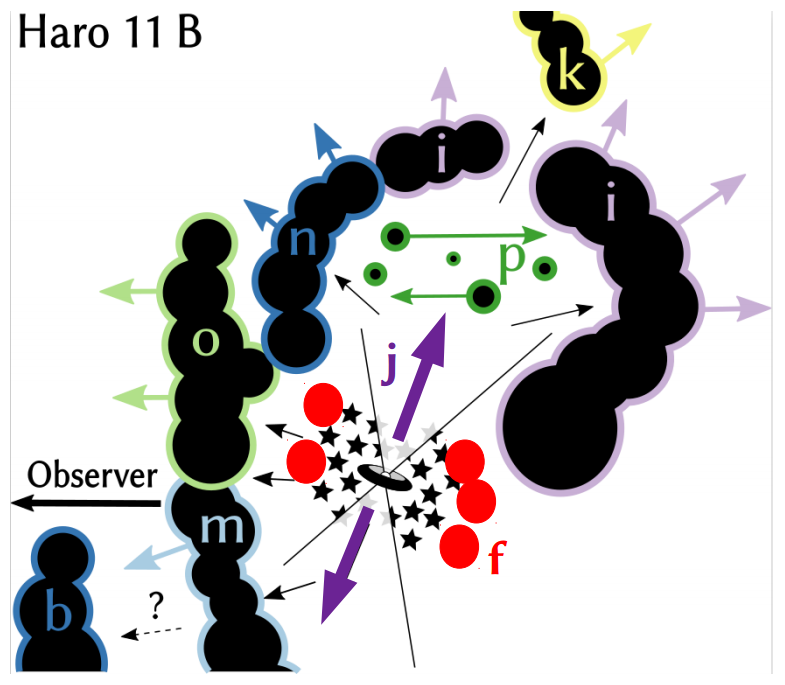
\includegraphics[width=0.23\textwidth]{Selection_205.png} 
   \caption{\small \textbf{Far left:} Slit position on Haro 11. To the right is
   knot B. \textbf{Center left:} Gaussian component centroids overlaid on 2D
   spectrum of H$\alpha$ in knot B., colored according to assigned label.
   \textbf{Center right:} BPT diagram of the central area around knot B.
   \textbf{Far right:} Explanatory sketch showing how a configuration of gas,
   starburst and a central low-luminosity AGN could give rise to a number of
   the observed components.}
   \label{fig:haro}
\end{figure}

The centroids of the result, for Haro 11 knot B, is shown in the center left
panel of Fig.~\ref{fig:haro}, with the $y$ axis being parallel to the slit
direction, and the $x$ axis parallel to the dispersion direction. The 2D
spectrum is shown under the centroids for comparison. Assuming that H$\alpha$
was present in all regions that also emitted in other strong lines (which turned
out to be a good approximation), we then used the H$\alpha$ line structure as a
template to fit a number of other lines, including H$\beta$ and a number of
forbidden metal lines, from which a number of diagnostics could then be computed
on a per-component and per-subsystem basis, as well as for the entire collapsed
spectrum for better comparison with values reported elsewhere in the literature.
This led to a very large and complex amount of computed and measured physical
properties in the galaxies, the interpretation of which is too complex and
voluminous to cover here. However, I do want to mention one result, partly
because it is exciting, partly because it shows off what the method can do. In
the usual BPT analysis, Haro 11 and both its single knots, are placed firmly
within the H\textsc{ii}/starburst type objects. However, the spatially resolved
BPT diagram of the central parts shown in the center-right panel of
fig.~\ref{fig:haro} shows that a couple of components/subsystems stick out,
especially the  red one (labeled $f$ in the paper). This, along with a number of
other pieces of circumstantial evidence, all pointed to a low-luminosity,
AGN-like object residing deep in the central starburst of knot B\footnote{More
detail can be found in these slides: \url{http://bit.ly/EsoHaroTalk}}.  The
far-right panel of Fig.~\ref{fig:haro} sketches how such a constellation of
starburst and LLAGN can reproduce a number of the kinematic components observed
in this region. It later turned out that this knot has been observed as a hard
X-Ray point source with the Chandra X-ray Observatory \citep{Grimes2007}. These
observations have been re-evaluated by \cite{Prestwich2015}, who concluded, from
the x-ray observations alone, that this object was consistent with a high-mass
X-Ray Binary seen under very specific circumstances, or with a slowly-accreting
intermediate-mass or supermassive black hole. The data have also been evaluated
by \cite{BasuZych2016} who likewise concluded that it is consistent with a
LLAGN-type object. We argue from the kinematics that the HMXB scenario is
unlikely, and conclude that it is more likely to be an accreting, massive Black
Hole. After the paper went into review, we have further discovered that one
component, $j$ in the sketch, is very strong in He\textsc{ii} 4686, with a
significant margin too strong to be due to massive stars; a further piece of
evidence supporting the LLAGN hypothesis. 


\section*{Future plans}

Apart from the opportunities offered as part of my future employments, these are
some projects that I currently am interested in pursuing.  \textbf{First}, I
have one more local galaxy suspected of housing a LLAGN-like object like that in
Haro 11, and it is observable from both Hawaii and Paranal, Chile. I am very
interested in applying for observing time at Keck/HIRES or VLT/X-Shooter or
similar instruments to test whether this galaxy does indeed contain this kind of
object.  \textbf{Second}, I wish to extend the work I did on LARS using a sample
of HST COS Legacy data from various samples of local starburst and compact dwarf
galaxies; and estimated $\sim 50$ such spectra are available publicly in the HST
archives. A standardized treatment of these could create a significantly
improved baseline for comparison with higher redshifts, as well as test already
found relations. \textbf{Third}, I am interested in combining the detailed
kinematic profile of H$\alpha$ (and thus the Ly $\alpha$ seed function) in Haro
11 knot B from submitted paper \emph{b}, with the observed Ly$\alpha$ profile
and neutral gas properties in submitted paper \emph{a}. The idea is still vague,
but comparison to simulations and radiative transfer models, combined with the
detailed knowledge we have of this galaxy, could help uncover how large a role
the intrinsic Ly $\alpha$ profile plays for the eventual escape fraction and
observed Ly$\alpha$ morphology etc. \textbf{Fourth}, I am CoI on a Cycle 24 HST
program in which 12 COS and 2 STIS pointings are placed on the nearby starburst
ESO 338, in essence using the COS as a coarse-grained, Far-UV IFU\@. We expect a
great wealth of information about ISM properties and Ly$\alpha$ radiative
transfer and escape to come from this project, and I have the opportunity to
lead at least one paper on this work. 
% \section{References/Citations}
\bibliographystyle{aasjournal} \begin{scriptsize} \begin{multicols}{2}
\bibliography{thesis} \end{multicols} \end{scriptsize}

%%% FIGURES GO HERE!!!
% \section*{Figures}
% 
% \begin{figure}[h] %  figure placement: here, top, bottom, or page
%    \centering
%    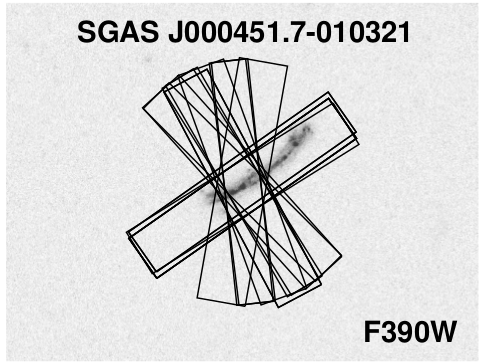
\includegraphics[width=0.39\textwidth]{MegasaurExample.png}
%    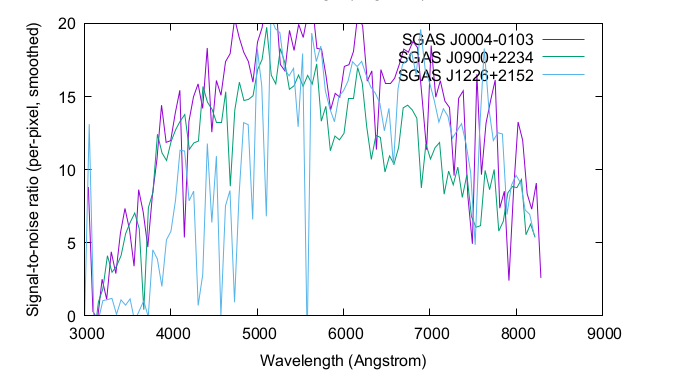
\includegraphics[width=0.59\textwidth]{SNRs.png} 
%    \caption{\small Example finding chart for Magellan/MagE observations of a Megasaur
% 	   (left), and averaged SNR per pixel in the combined spectra of same
% 	   galaxy (purple) and two other sample galaxies (right). Images 
% 	   provided by J. Rigby.}
%    \label{fig:mega}
% \end{figure}
% 
% 
% \begin{figure}[h] %  figure placement: here, top, bottom, or page
%    \centering
%    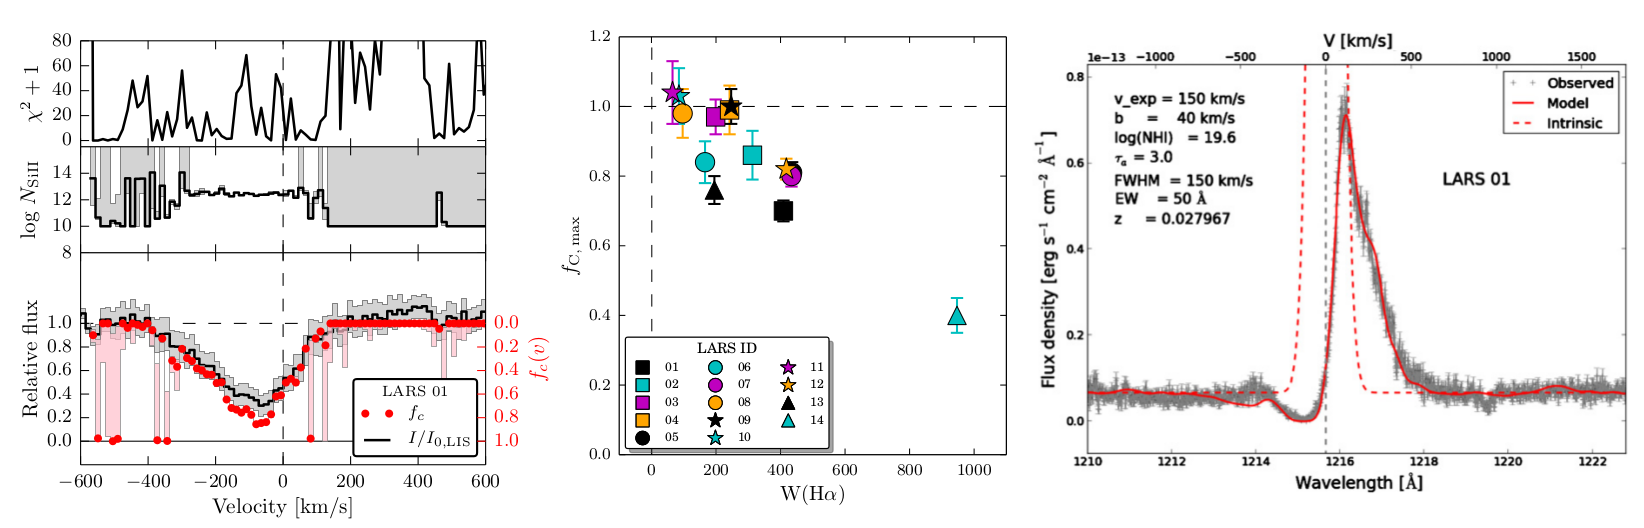
\includegraphics[width=\textwidth]{LarsResults.png} 
%    \caption{\small eft: Result of Apparent Optical Depth analysis of a LARS galaxy.
%    Middle panel shows inferred column densities with errors, lower panel
%    shows computed values of $f_C$ (see sect. \ref{sec:weird}), overlaid on the
%    averaged LIS metal absorption profile; from RT15. Center: H$\alpha$ EW vs.
%    Maximum covering fraction for the LARS galaxies; from RT15. Right: Ly$\alpha$
%    profile of LARS 1 (black), with intrinsic Ly$\alpha$ inferred from H$\alpha$
%    (dotted red) and the best-fit model from the catalog of the Geneva group
%    (Orlitova et al, in prep.), from \cite{LARSI}.}
%    \label{fig:LARS}
% \end{figure}
% 
% 
% \begin{figure}[h] %  figure placement: here, top, bottom, or page
%    \centering
%    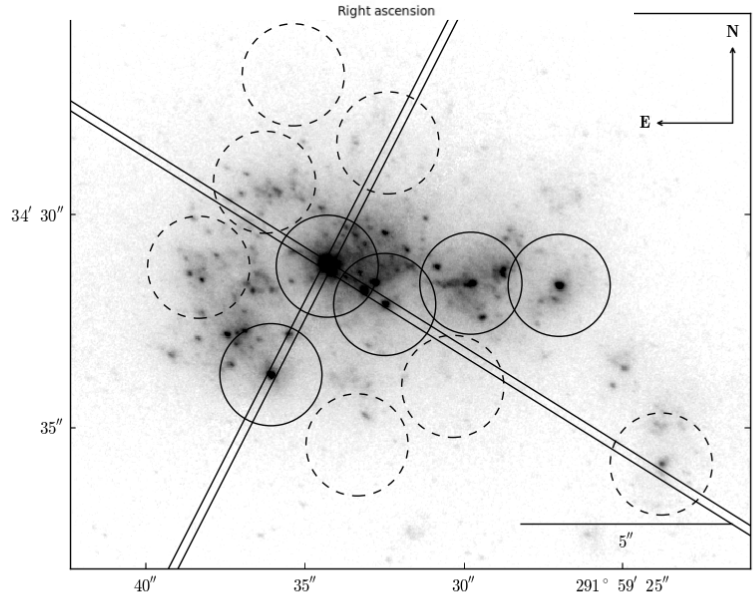
\includegraphics[width=3.0in]{SAFEpointings.png} 
%    \caption{STIS and COS pointings for the SAFE project., overlaid on HST UV
%    continuum image of ESO 338-04. Image from SAFE proposal by Östlin.}
%    \label{fig:example}
% \end{figure}
% 
% % \begin{figure}[h] %  figure placement: here, top, bottom, or page
% %    \centering
% %    \includegraphics[width=\textwidth]{../../../Haro11Cos/Figs/AOD-details-example-4pane.pdf} 
% %    \caption{Illustration of the AOD method with example data from Haro 11.
% %    \textbf{Far left}: Line profile of Si\textsc{ii}\(\lambda\lambda 1260, 1304,
% %    1526\), and a vertical red line denoting the velocity bin of interest for the
% %    example. \textbf{Center left}: Residual intensity as a function of
% %    \(f\lambda\) for the three lines. The best fit of \(I/I_0(f\lambda)\) is 
% %    shown in magenta. In gray is shown for illustration \(I/I_0\) in the extreme
% %    cases of \emph{a)} unchanged $f_C$ but much higher $N$ (dotted) or \emph{b)}
% %    $f_C=1$ and $N$ 0.5 dex lower. \textbf{Center right}: $\log N$ as function of
% %    $v$ for these profiles, and \textbf{far right}: $1-f_C$ as function of v
% %    (orange circles) superimposed on the profile of Si \textsc{ii} 1260 (black
% % 	   steps). Shaded regions are standard errors. }
% %    \label{fig:example}
% % \end{figure}


\end{document}  
